%%%%%%%%%%%%%%%%%%%%%%%%%%%%%%%%%%%%%%%%%
% a0poster Portrait Poster
% LaTeX Template
% Version 1.0 (22/06/13)
%
% The a0poster class was created by:
% Gerlinde Kettl and Matthias Weiser (tex@kettl.de)
% 
% This template has been downloaded from:
% http://www.LaTeXTemplates.com
%
% License:
% CC BY-NC-SA 3.0 (http://creativecommons.org/licenses/by-nc-sa/3.0/)
%
%%%%%%%%%%%%%%%%%%%%%%%%%%%%%%%%%%%%%%%%%

%----------------------------------------------------------------------------------------
%	PACKAGES AND OTHER DOCUMENT CONFIGURATIONS
%----------------------------------------------------------------------------------------

\documentclass[a0,portrait]{a0poster}

\usepackage{multicol} % This is so we can have multiple columns of text side-by-side
\columnsep=100pt % This is the amount of white space between the columns in the poster
\columnseprule=3pt % This is the thickness of the black line between the columns in the poster

\usepackage[svgnames]{xcolor} % Specify colors by their 'svgnames', for a full list of all colors available see here: http://www.latextemplates.com/svgnames-colors

\usepackage{times} % Use the times font
%\usepackage{palatino} % Uncomment to use the Palatino font

\usepackage{graphicx} % Required for including images
\graphicspath{{figures/}} % Location of the graphics files
\usepackage{textcomp}
\usepackage{bm}
\usepackage[round]{natbib}
\usepackage{caption}
\usepackage{subfig}
\usepackage{listings}
\usepackage{hyperref}
\usepackage{pgfplots}
\usepackage{tikz}
\usepackage{amsthm}
\usepackage{pgf,pgfarrows,pgfnodes}
\usepackage{amsmath}
\usepackage{amsfonts}
\usepackage{amssymb}
\usepackage{booktabs}       % professional-quality tables
\usepackage{wrapfig}
\usepackage{indentfirst}
\usepackage{setspace}
\usepackage{graphicx}
\usepackage{textcomp}
\usepackage{array}
\usetikzlibrary{fit}
\usetikzlibrary{arrows.meta}
\usepackage{array, multirow}
\usepackage{booktabs} % Top and bottom rules for table
\usepackage[font=small,labelfont=bf]{caption} % Required for specifying captions to tables and figures
\usepackage{amsfonts, amsmath, amsthm, amssymb} % For math fonts, symbols and environments
\usepackage{wrapfig} % Allows wrapping text around tables and figures
\newcommand{\norm}[1]{\left\lVert#1\right\rVert}
\newcommand{\rank}{r}
\DeclareMathOperator{\ttrank}{TT-rank}
\DeclareMathOperator{\ttround}{TT-round}
\DeclareMathOperator{\grad}{grad}
\renewcommand{\vec}[1]{\boldsymbol{#1}}
\newcommand{\tens}[1]{\boldsymbol{\mathcal{#1}}}
\newcommand{\tensel}[1]{\mathcal{#1}}
\newcommand{\GP}{\mathcal{GP}}
\newcommand{\E}{\mathbb{E}}
\newcommand{\R}{\mathbb{R}}
\newcommand{\N}{\mathcal{N}}
\newcommand{\bigO}{\mathcal{O}}
\newcommand{\cov}{\mbox{cov}}
\newcommand{\KL}[2]{\mbox{KL}\left(#1\mbox{ || }#2\right)}
\newcommand{\tr}{\mbox{tr}}
\graphicspath{{pics/tt/}}
\newcommand{\includesvg}[1]{%
    \executeiffilenewer{#1.svg}{#1.pdf}%
      {inkscape -z -D --file=#1.svg %
      --export-pdf=#1.pdf --export-latex}%
      \input{#1.pdf_tex}%
      }
\newcommand{\executeiffilenewer}[3]{%
  \ifnum\pdfstrcmp{\pdffilemoddate{#1}}%
  {\pdffilemoddate{#2}} > 0 {\immediate\write18{#3}}\fi}


\begin{document}

%----------------------------------------------------------------------------------------
%	POSTER HEADER 
%----------------------------------------------------------------------------------------

% The header is divided into two boxes:
% The first is 75% wide and houses the title, subtitle, names, university/organization and contact information
% The second is 25% wide and houses a logo for your university/organization or a photo of you
% The widths of these boxes can be easily edited to accommodate your content as you see fit

%\begin{minipage}[b]{0.25\linewidth}
%\begin{center}
%  \centering
%
\includegraphics[width=10cm]{pics/logos/bayesgroup.pdf}
% \vspace{0.5cm}
%\end{center}
%\end{minipage}
%\begin{minipage}[b]{0.25\linewidth}
%\begin{center}
%  \centering
%  
\includegraphics[width=7cm]{pics/logos/msu_blue.eps}
%\end{center}
% \vspace{0.5cm}
%\end{minipage}
%\begin{minipage}[b]{0.25\linewidth}
%\begin{center}
%  \centering
%
\includegraphics[width=7cm]{pics/logos/cornell.png}
%\end{center}
%\end{minipage}
%\begin{minipage}[b]{0.25\linewidth}
%\begin{center}
%  \centering
%  
\includegraphics[width=7cm]{pics/logos/hse.pdf}
%\end{center}
%\end{minipage}

\begin{minipage}[b]{.75\linewidth}
  \begin{center}
  \veryHuge \color{NavyBlue} 
    \textbf{Scalable Gaussian Processes with Billions of\\ Inducing Inputs \\via Tensor Train Decomposition} \color{Black}\\ % Title
    {
      \huge 
      \renewcommand{\arraystretch}{0.5}
      \begin{tabular}{c}
        \textbf{Pavel Izmailov}\\
        {\Large \texttt{pi49@cornell.edu}}
      \end{tabular}\quad 
      \begin{tabular}{c}
        \textbf{Alexander Novikov}\\
        {\Large \texttt{sasha.v.novikov@gmail.com}}
      \end{tabular}
      \quad 
      \begin{tabular}{c}
        \textbf{Dmitry Kropotov}\\
        {\Large \texttt{dmitry.kropotov@gmail.com}}
      \end{tabular}
      %\\[0.5cm] % Author(s)
    }
  %\huge \textbf{Pavel Izmailov\textsuperscript{1,4} \quad Alexander Novikov\textsuperscript{2,3} \quad Dmitry Kropotov\textsuperscript{4}}\\[0.5cm] % Author(s)
%\Large \textsuperscript{1} Cornell University 
%  \quad 
%  \textsuperscript{2} National Research University Higher School of Economics\\
%  \quad 
%  \textsuperscript{3} Institute of Numerical Mathematics RAS
%  \quad 
%  \textsuperscript{4} Lomonosov Moscow State University
%  \\[0.4cm] % University/organization
\end{center}
\end{minipage}
\begin{minipage}[b]{0.25\linewidth}
  \begin{minipage}[b]{0.49\linewidth}
  \begin{center}
    \centering
  
\includegraphics[width=10cm]{pics/logos/bayesgroup.pdf}
  \vspace{0.5cm}
  \end{center}
  \end{minipage}
  \begin{minipage}[b]{0.49\linewidth}
  %\hspace{1cm}
  \begin{center}
    \centering
    
\includegraphics[width=7cm]{pics/logos/msu_blue.eps}
  \end{center}
  \vspace{0.5cm}
  \end{minipage}
  \begin{minipage}[b]{0.49\linewidth}
  \begin{center}
    \centering
  
\includegraphics[width=7cm]{pics/logos/cornell.png}
  \end{center}
  \end{minipage}
  \begin{minipage}[b]{0.49\linewidth}
  \begin{center}
    \centering
    
\includegraphics[width=7cm]{pics/logos/hse.pdf}
  \end{center}
  \end{minipage}
\end{minipage}

%\vspace{1cm} % A bit of extra whitespace between the header and poster content
\large

%----------------------------------------------------------------------------------------

\begin{multicols}{2} % This is how many columns your poster will be broken into, a portrait poster is generally split into 2 columns

%----------------------------------------------------------------------------------------
%	ABSTRACT
%----------------------------------------------------------------------------------------

%\begin{abstract}
%
%Abstract
%\end{abstract}

\section*{\LARGE \color{NavyBlue}Summary}

\begin{itemize}
  \item Gaussian processes are powerful and elegant models, but exact inference 
    requires $\bigO(n^3)$ computations, where $n$ is the number of training data
  \item We propose the Tensor Train GP (TT-GP) framework with 
    linear complexity  $\bigO(n)$ 
  \item TT-GP allows to build flexible posterior approximations and train
    expressive deep kernels by using billions of inducing points for datasets
    containing millions of data points of dimensionality up to $10$
  \item TT-GP achieves state-of-the-art results on several important benchmarks
    both with RBF and deep kernels
\end{itemize}

\section*{\LARGE \color{NavyBlue}Inducing Inputs and Structured Kernel Interpolation}

\begin{itemize}
  \item Inducing inputs are imaginary data points that allow to speed up GP inference
  \item SKI \citep{wilson2015}: set inducing points on a multi-dimensional grid
    \[
      Z = Z^1 \times Z^2 \times \ldots \times Z^D.
    \]
  
  \item Assume the kernel decomposes as
    \[
      k(x, x') = k^1(x^1, x'^1) \cdot k^2(x^2, x'^2) \cdot \ldots \cdot k^D(x^D, x'^D)
    \]
    Covariance matrix $K_{mm} \in \R^{m \times m}$ computed at the
    inducing points takes form
    \[
      K_{mm} = K_{m_1 m_1}^1 \otimes K_{m_2 m_2}^2 \otimes \ldots \otimes K_{m_D m_D}^D
    \] 

\end{itemize}
\begin{minipage}[b]{0.45\linewidth}

  \begin{center}
    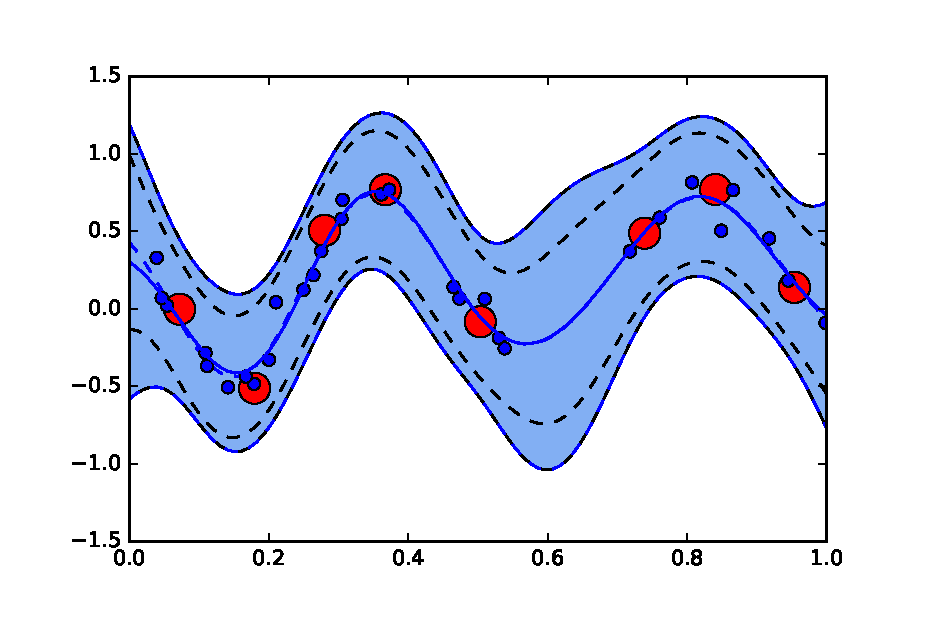
\includegraphics[width=1.\linewidth]{pics/gps/1d_gp_ind_inputs.eps}
  \end{center}

  \vspace{-1cm}
\end{minipage}
\begin{minipage}[b]{0.5\linewidth}
  \begin{center}
    \centering
    \scalebox{1.25}{
      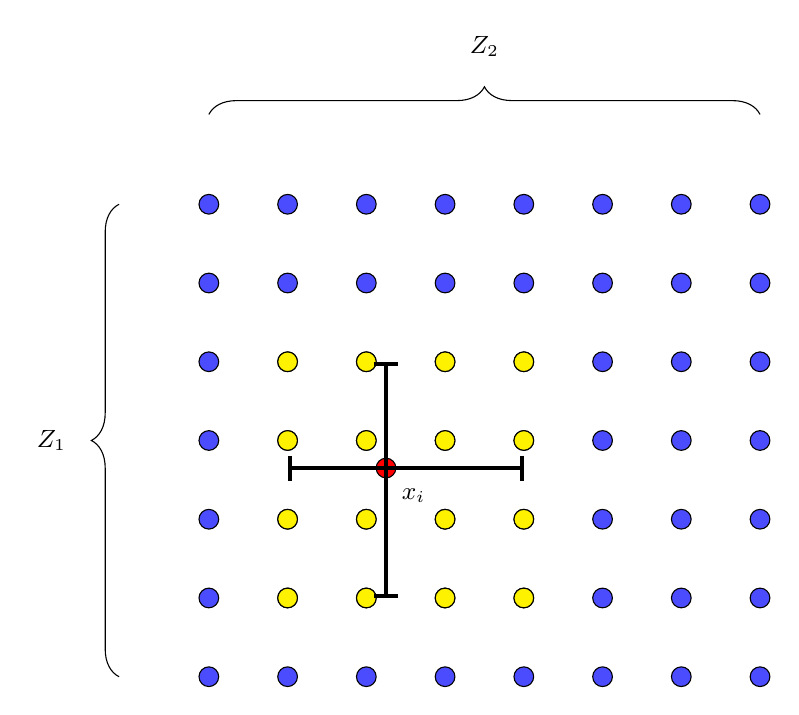
\begin{tikzpicture}
	
  \foreach \x in {1, 2, 3, 4, 5, 6, 7, 8} 
    \foreach \y in {1, 2, 3, 4, 5, 6, 7} 
      \node[circle, draw, fill=blue!70, inner sep=0pt, minimum size=0.25cm] at (\x, \y) {};

    
  \foreach \x in {2, 3, 4, 5} 
    \foreach \y in {2, 3, 4, 5} 
      \node[circle, draw, fill=yellow, inner sep=0pt, minimum size=0.25cm] at (\x, \y) {};

  \draw [decorate,decoration={brace,amplitude=10pt,raise=4pt},yshift=0pt]
    (0, 1) -- (0,7) node [black,midway,xshift=-1.cm] 
    {\small $Z_1$};

  \draw [decorate,decoration={brace,amplitude=10pt,raise=4pt},yshift=0pt]
    (1, 8) -- (8, 8) node [black,midway,yshift=1.cm] {\small $Z_2$};

  \node[circle, draw, fill=red, inner sep=0pt, minimum size=0.25cm] at (3.25, 3.65) {};
  \node[] at (3.6, 3.3) {\small $x_i$};
  \draw[|-|, line width=1.5pt] (3.25, 2) to (3.25, 5);
  \draw[|-|, line width=1.5pt] (2, 3.65) to (5, 3.65);

\end{tikzpicture}

    }
  \end{center}
\end{minipage}
    
    \begin{itemize}
      \item $\det(K_{mm})$ and $K_{mm}^{-1}$ can be computed efficiently
      \item Inducing points can be considered as inteprolation points for the
        kernel
        \[
          k_i \approx K_{mm} w_i,
        \]
      where $k_i \in \R^m$ is the vector of covariances between the $i$-th training
      object and the inducing points, $w_i\in \R^{m}$ is the vector of interpolation coefficients

      \item KISS-GP uses cubic convolutional interpolation for which 
        \[
          w_i = w_i^1 \otimes w_i^2 \otimes \ldots \otimes w_i^D
        \]
\end{itemize}

\section*{\LARGE \color{NavyBlue} Tensor Train Format}

Tensor $\tens{A}$ is said to be represented in Tensor Train \citep{oseledets2011}  format if:
\vspace{0.2cm}
\flushleft
\def\svgwidth{33cm}
\includesvg{pics/tt/TT}

\begin{itemize}
  \item TT-format uses $O \left ( d n r^2 \right )$ memory to approximate a
    tensor with $n^d$ elements
  \item Allows for efficient implementation of linear algebra operations
\end{itemize}


\section*{\LARGE \color{NavyBlue}Gaussian Process ELBO}
    
Evidence Lower Bound \citep{hensman2013} with KISS-GP approximation of $k_i$:
%$k_i \approx K_{mm} w_i$:
\[
  \log p(y) \ge \sum_{i=1}^n \bigg(\log \N (y_i | w_i^T \mu, \sigma^2) - 
  \frac 1 {2 \sigma^2} (\delta - k_i^T K_{mm}^{-1} k_i) - \frac 1 {2 \sigma^2} 
    \tr (w_i^T \Sigma w_i)\bigg)
\]
\[
  - \frac 1 2 \bigg(\log \frac {\det (K_{mm})} {\det (\Sigma)} - m + \tr(K_{mm}^{-1} \Sigma)
  + \mu^T K_{mm}^{-1}\mu \bigg)
\]
where
\begin{itemize}
%  \item $K_{mm} \in \R^{m \times m}$ is the covariance matrix computed at the
%    inducing points
%  \item $k_i \in \R^m$ is the vector of covariances between the $i$-th training
%    object and the inducing points
  \item $\sigma^2$ is the noise variance
  \item $\delta$ is the prior variance of the process at any point
  \item $\mu \in \R^m$, $\Sigma \in \R^{m \times m}$ — variational parameters
  %\item $\delta_{i} = \delta - k_i^T K_{mm}^{-1} k_i$, where  
  %  $\delta$ is the prior variance of the process at any point
\end{itemize}

\section*{\LARGE \color{NavyBlue}TT-GP}

\begin{itemize}
  \item Set inducing points $Z$ on a grid in the feature space
  \item Restrict $\Sigma$ to be in a Kronecker product format
    \[
      \Sigma = \Sigma^1 \otimes \Sigma^2\otimes \ldots \otimes \Sigma^D
    \]
  \item Represent $\mu$ as a $d$-dimensional tensor, restrict to be in TT format
    with TT-ranks $r$
  \item Maximize ELBO with respect to TT-cores of $\mu$, Kronecker factors of 
    $\Sigma$ using SGD
\end{itemize}

\section*{\LARGE \color{NavyBlue} Properties}
    
\begin{itemize}
  \item Linear computational complexity in the size of the data
    $\bigO(n D m^{1 / D} r^2 + D m^{1 / D} r^3 + D m^{3 / D})$. 
    TT-ranks are in general on the scale of $r \approx 10$.\\ 
    Here $m = m_0^D$
  \item TT-GP can be applied for very large $n$ and $m$
\end{itemize}

\section*{\LARGE \color{NavyBlue} RBF Kernel Experiments}

Comparison with SVI-GP \citep{hensman2013} on regression and classification
tasks:

\begin{center}
  \begin{tabular}{lll l cll l clll}
    \toprule
    \multicolumn{3}{c}{Dataset} && \multicolumn{3}{c}{SVI-GP / KLSP-GP} && \multicolumn{4}{c}{TT-GP} \\
    \cmidrule{1-3}
    \cmidrule{5-7}
    \cmidrule{9-12}

    Name & $n$ & $D$ &&
    acc. & $m$ & $t$ (s) &&
    acc. & $m$ & $d$ & $t$ (s)\\
    \midrule

    Powerplant & $7654$ & $4$ &&
    $0.94$ & $200$ & $10$ &&
    $\mathbf{0.95}$ & $35^4$ & - & $5$ \\

    Protein & $36584$ & $9$ &&
    $0.50$ & $200$ & $45$ &&
    $\mathbf{0.56}$ & $30^9$ & - & $40$ \\

    YearPred & $463K$ & $90$ &&
    $0.30$ & $1000$ & $597$ &&
    $\mathbf{0.32}$ & $10^6$ & $6$ & $105$ \\

    \midrule
    Airline & $6M$ & $8$ &&
    $0.665^*$ & - & - &&
    $\mathbf{0.694}$ & $20^8$ & - & $5200$ \\

    svmguide1 & 3089 & 4 &&
    $0.967$ & $200$ & $4$ &&
    $\mathbf{0.969}$ & $20^4$ & - & $1$\\

    EEG & 11984 & 14 &&
    $\mathbf{0.915}$ & $1000$ & $18$ &&
    $0.908$ & $12^{10}$ & $10$ & $10$\\

    covtype bin & 465K & 54 &&
    $0.817$ & $1000$ & $320$ &&
    $\mathbf{0.852}$ & $10^6$ & $6$ & $172$\\
    \bottomrule
  \end{tabular}
\end{center}
\section*{\LARGE \color{NavyBlue} Deep Kernel Experiments}
    
Embedding learned by TT-GP with a deep kernel on {\it digits}
dataset:

\begin{center}
    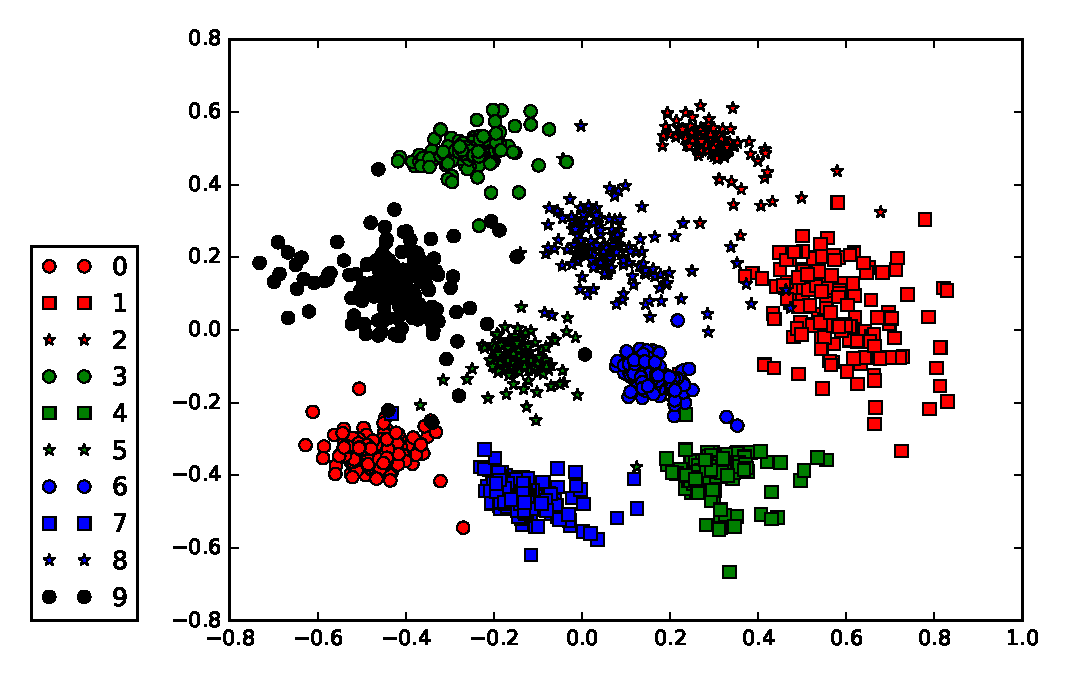
\includegraphics[width=20cm]{pics/embed/embedding_2.eps}
\end{center}

Comparison with SV-DKL \citep{wilson2016stochastic} and stand-alone
DNN:

\begin{center}
    \label{deep_results}
    \centering
    \begin{tabular}{lll ll llll lll}
      \toprule
      \multicolumn{2}{c}{Dataset}  && SV-DKL &&
      \multicolumn{2}{c}{DNN} &&
      \multicolumn{3}{c}{TT-GP}\\

      \cmidrule{1-2}
      \cmidrule{4-4}
      \cmidrule{6-7}
      \cmidrule{9-11}

      Name & n &&
      acc. && acc. & $t$ (s) &&
      acc. & $d$ & $t$ (s)
      \\
      \midrule


      %\cmidrule{9-10}
      %\cmidrule{12-13}

      Airline & $6M$ && 
      $0.781$ && $0.780$ & $1055$ &&
      $\mathbf{0.788 \pm 0.002}$ & $2$ & $1375$\\

      CIFAR-10 & $50 K$ && 
      $-$ && $\mathbf{0.915}$ & $166$ &&
      $0.908 \pm 0.003$ & $9$ & $220$\\

      MNIST & $60K$ && 
      $-$ && $0.993$ & $23$ &&
      $\mathbf{0.9936 \pm 0.0004}$ & $10$ & $64$\\
      \bottomrule
    \end{tabular}
\end{center}


%\nocite{*} % Print all references regardless of whether they were cited in the poster or not
%\bibliographystyle{plain} % Plain referencing style
\bibliography{biblio} % Use the example bibliography file sample.bib
\bibliographystyle{plainnat}

%\section*{Acknowledgements}


\end{multicols}
\end{document}
